\documentclass[10pt,pdf,hyperref={unicode}]{beamer} %aspectratio=169-для 16:9
\usepackage[T2A]{fontenc}
\usepackage[utf8]{inputenc}
\usepackage[english,russian]{babel} 
\usepackage{amssymb,amsfonts,amsmath,mathtext}
\usepackage{cite,enumerate,float,indentfirst}
\usepackage{graphicx}
\usepackage{multimedia}
\usepackage{hyperref}
\usepackage{pgfplots}
\usepackage{pgfplotstable}
\usepackage{subfig}

\renewcommand{\rmdefault}{ftm}

\addto\captionsrussian{%
\renewcommand{\figurename}{}%
\renewcommand{\tablename}{}%
}

\graphicspath{{fig/}}

\usetheme{Boadilla}
\usecolortheme{crane}
%\usefonttheme[onlylarge]{structurebold}
\usefonttheme[onlymath]{serif}
\setbeamerfont{institute}{size=\normalsize}
\setbeamercolor{color1}{bg=blue!60!black,fg=white}
\beamertemplatenavigationsymbolsempty

\makeatletter
\defbeamertemplate*{footline}{my theme}{
    \leavevmode
    \hbox{
    \begin{beamercolorbox}[wd=\paperwidth,ht=2.25ex,dp=1ex,right]{date in head/foot}
        \insertframenumber{} / \inserttotalframenumber \hspace*{2ex}
    \end{beamercolorbox}}
}
\makeatother

\title{ Решение задач трехфазной неизотермической фильтрации \\
на высокопроизводительных вычислительных системах}
\author{Люпа Анастасия Александровна}
\institute{Московский физико-технический институт \\
(государственный университет)\\
%\vspace{0.1cm}
Факультет управления и прикладной математики \\
Кафедра математического моделирования \\
    \vspace{0.2cm}
    Научный руководитель: с.н.с., к.ф.-м.н. Чурбанова Н.Г.\\
}
\date{
    Москва 2014г.
}

\begin{document}

\begin{frame}
  \maketitle
\end{frame}

\section{Содержание}

\begin{frame}
\begin{center}
\frametitle{Содержание}
\framesubtitle{\ }
\begin{itemize}
\item {\large Введение}
\vspace{0.3cm}
\item {\large Цели работы}
\vspace{0.3cm}
\item {\large Математическая модель трехфазной фильтрации}
\vspace{0.3cm}
\item {\large Алгоритм расчета модели}
\vspace{0.3cm}
\item {\large Параллельная реализация алгоритма}
\vspace{0.3cm}
\item {\large Тестовые задачи}
\vspace{0.3cm}
\item {\large Анализ производительности вычислений}
\vspace{0.3cm}
\item {\large Заключение}
\end{itemize}
\end{center}
\end{frame}

\section{Введение}

\begin{frame}
\begin{center}
\frametitle{Введение}
\framesubtitle{\ }
\begin{figure}
\begin{minipage}[h]{0.43\textwidth}
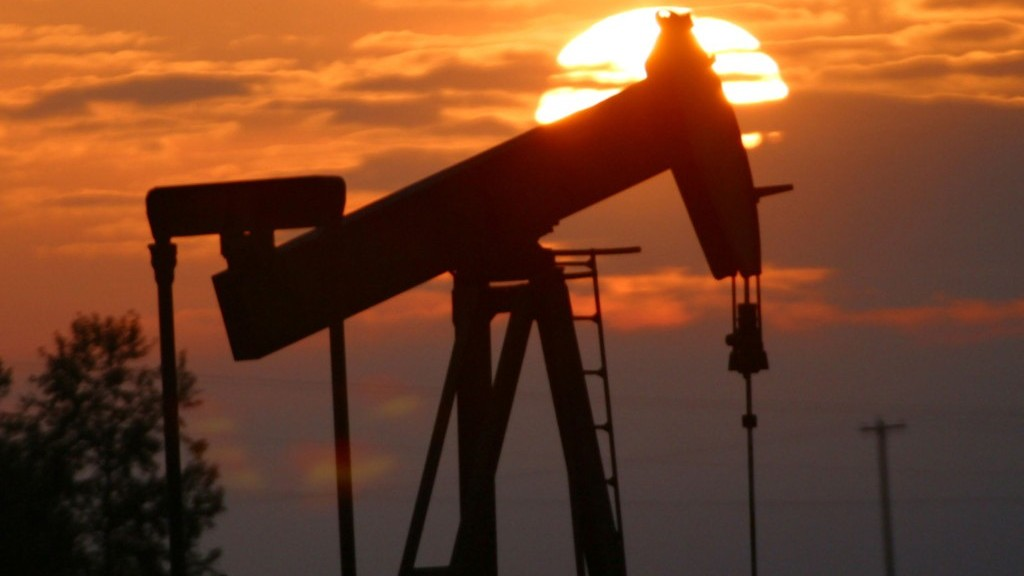
\includegraphics[width=1.0\textwidth]{oil_pump169.jpg}
\caption{\small{Добыча нефти и газа\\ \ }}
\end{minipage}
\hspace{8mm}
\begin{minipage}[h]{0.43\textwidth}
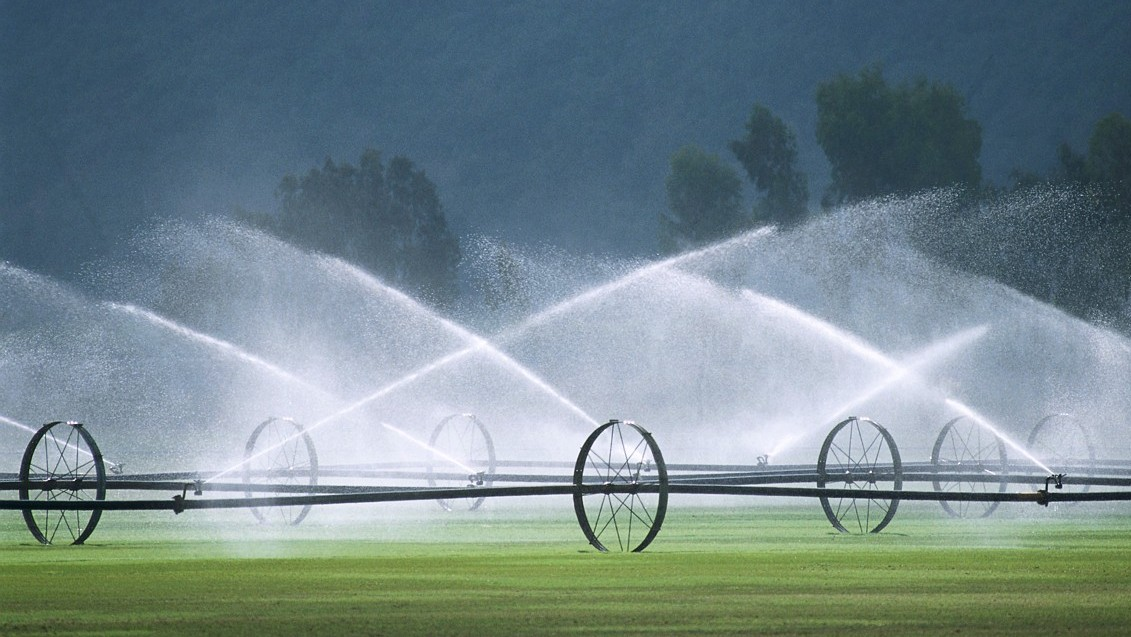
\includegraphics[width=1.0\textwidth]{melio169.jpg}
\caption{\small{Мелиоративные сооружения\\ \ }}
\end{minipage}
\vfill
\begin{minipage}[h]{0.43\textwidth}
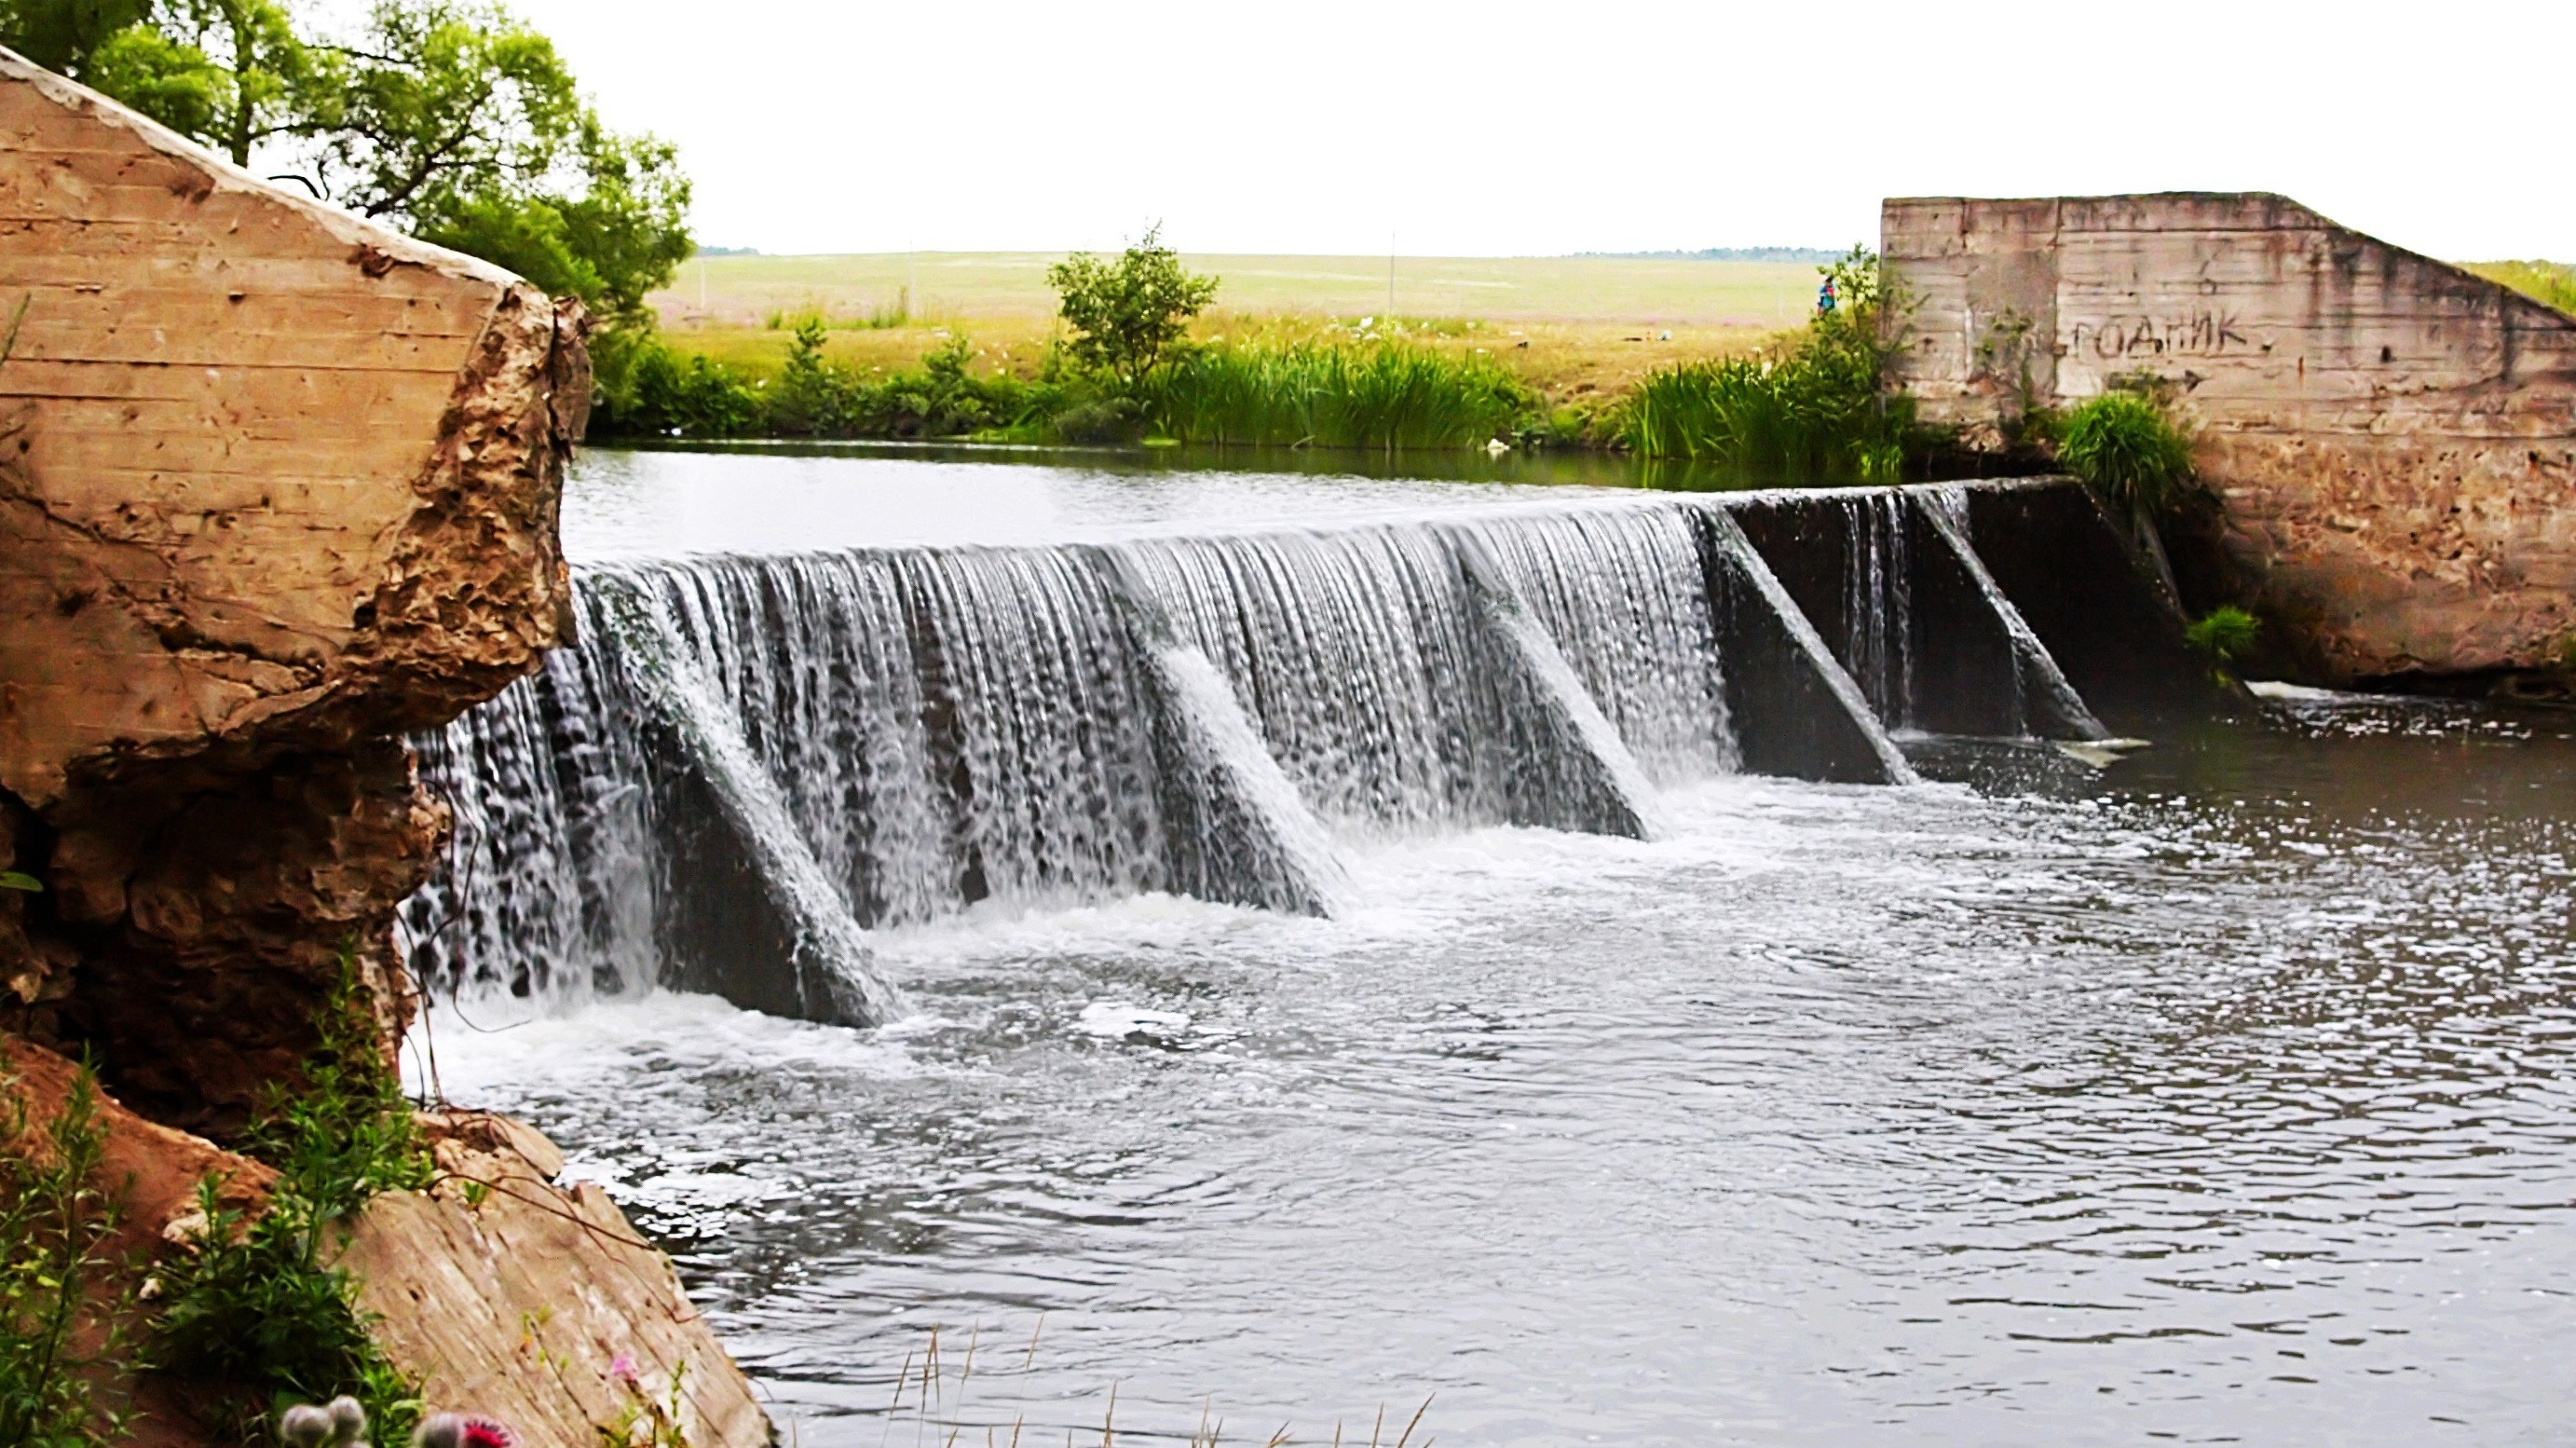
\includegraphics[width=1.0\textwidth]{plotina169.jpg}
\caption{\small{Гидротехнические сооружения}}
\end{minipage}
\hspace{8mm}
\begin{minipage}[h]{0.43\textwidth}
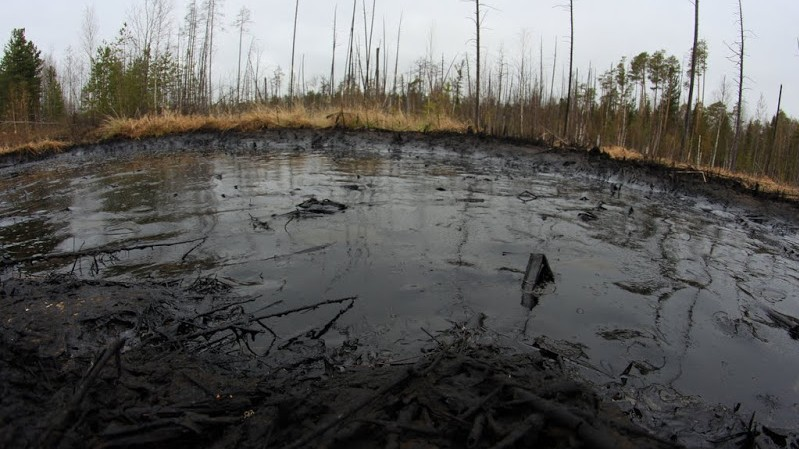
\includegraphics[width=1.0\textwidth]{dirty169.jpg}
\caption{\small{Решение экологических проблем}}
\end{minipage}
\end{figure}
\end{center}
\end{frame}

\section{Цели работы}

\begin{frame}
\begin{center}
\frametitle{Цели работы}
\framesubtitle{\ }
\begin{itemize}
\item {\large Построение математической модели трехфазной неизотермической фильтрации в пористой среде, допускающей реализацию явными методами\\}
\vspace{0.5cm}
\item {\large Создание алгоритмов и программ, ориентированных на гибридные кластеры с графическими ускорителями\\}
\vspace{0.5cm}
\item {\large Проведение тестовых расчетов}
\end{itemize}
\end{center}
\end{frame}

\section{Математическая модель трехфазной фильтрации}

\begin{frame}
\begin{center}
\frametitle{Математическая модель трехфазной фильтрации}
\framesubtitle{Основные предположения}
\begin{itemize}
\item Трехфазные течения: вода, легкая нефть и газ
\vspace{0.3cm}
\item Фазы несмешивающиеся
\vspace{0.3cm}
\item Жидкости слабосжимаемые
\vspace{0.3cm}
\item Газ идеальный
\vspace{0.3cm}
\item Среда пористая, однородная, изотропная, неподвижная
\vspace{0.3cm}
\item Учитываются капиллярные силы и гравитационное поле
\vspace{0.3cm}
\item Учитываются тепловые процессы
\end{itemize}
\end{center}
\end{frame}

\begin{frame}
\begin{center}
\frametitle{Математическая модель трехфазной фильтрации}
\framesubtitle{Полная система уравнений}
\begin{equation*}
\left\{
  \begin{aligned}
    & \text{1)}\ \frac{\partial \left(m {\sum\limits_{i}{\rho_i S_i E_i(P_i, T)}} + (1-m){\rho_r E_r(P_w, T)}\right)}{\partial t} + \\
    & \qquad + div(\sum_{i}{\rho_i H_i(T) \overrightarrow{u_i}}) = div(\lambda_{eff} grad T),\\
    & \text{2)}\ \frac{\partial (m \rho_i S_i)}{\partial t}+ div(\rho_i \overrightarrow{u_i}) = \rho_i q_i,\\
    & \text{3)}\ \overrightarrow{u_i}=-K \frac{k_i}{{\mu_i(T)}}(grad P_i - {\rho}_i\overrightarrow{g}),\\
    & \text{4)}\ S_w + S_n + S_g=1,\\
    & \text{5)}\ P_n=P_w+P_{cnw}(\overline{S_w}),\quad P_g=P_w+P_{cnw}(\overline{S_w})+P_{cgn}(\overline{S_g}),\\
    & \text{6)}\ k_w=k_w(\overline{S_w}),\quad k_g=k_g(\overline{S_g}),\quad k_n=k_n(\overline{S_w},\overline{S_n}),\\
    & \text{7)}\ \rho_i=\rho_i(P_i,T),\\
    &i=w,n,g. \\
  \end{aligned}
\right.
\end{equation*}
\end{center}
\end{frame}

\begin{frame}
\begin{center}
\frametitle{Математическая модель трехфазной фильтрации}
\framesubtitle{Полная система уравнений с модифицированным уравнением неразрывности}
\begin{equation*}
\left\{
  \begin{aligned}
    & \text{1)}\ \frac{\partial \left(m {\sum\limits_{i}{\rho_i S_i E_i(P_i, T)}} + (1-m){\rho_r E_r(P_w, T)}\right)}{\partial t} + \\
    & \qquad + div(\sum_{i}{\rho_i H_i(T) \overrightarrow{u_i}}) = div(\lambda_{eff} grad T),\\
    & \text{2)}\ \frac{\partial (m \rho_i S_i)}{\partial t}+ div(\rho_i \overrightarrow{u_i}) = \rho_i q_i\textcolor{red}{ + l c_i \cdot div(grad(\rho_i S_i))}, \\
    & \text{3)}\ \overrightarrow{u_i}=-K \frac{k_i}{{\mu_i(T)}}(grad P_i - {\rho}_i\overrightarrow{g}),\\
    & \text{4)}\ S_w + S_n + S_g=1,\\
    & \text{5)}\ P_n=P_w+P_{cnw}(\overline{S_w}),\quad P_g=P_w+P_{cnw}(\overline{S_w})+P_{cgn}(\overline{S_g}),\\
    & \text{6)}\ k_w=k_w(\overline{S_w}),\quad k_g=k_g(\overline{S_g}),\quad k_n=k_n(\overline{S_w},\overline{S_n}),\\
    & \text{7)}\ \rho_i=\rho_i(P_i,T),\\
    &i=w,n,g. \\
  \end{aligned}
\right.
\end{equation*}
\end{center}
\end{frame}

\section{Алгоритм расчета модели}

\begin{frame}
\begin{center}
\frametitle{Алгоритм расчета модели}
\framesubtitle{\ }
\begin{enumerate} 
\item Применение граничных условий.
\item Вычисление давлений $P_n$,
$P_g$ через $P_w$ и капиллярные давления. 
\item Вычисление плотностей фаз. 
\item
Нахождение относительных фазовых проницаемостей фаз и~вязкости.
\item Определение
коэффициентов в~законе Дарси для~фаз. 
\item 
\label{roS} 
Нахождение ${\rho}_iS_i$ на~
следующем шаге по времени из~уравнения неразрывности явным численным методом.
\item 
\label{roE} 
Нахождение внутренней энергии системы на~
следующем шаге по~времени из~уравнения сохранения энергии явным численным методом.
\item 
\label
{Newton} Решение нелинейной системы из~пяти уравнений методом Ньютона,
в результате чего находим $P_w$, $S_w$, $S_n$, $S_g$, $T$ на следующем шаге по~времени.
\item Сохранение полученных значений переменных в~текстовый файл
в~формате, подходящем для~визуализации.
\item Обмены данными при~многопроцессорных вычислениях.
\end{enumerate} 
\end{center}
\end{frame}

\section{Параллельная реализация алгоритма}

\begin{frame}
\begin{center}
\frametitle{Параллельная реализация алгоритма}
\framesubtitle{\ }
\end{center}
\end{frame}

\begin{frame}
\begin{center}
\frametitle{Параллельная реализация алгоритма}
\framesubtitle{Комплекс программ}
\begin{itemize}
\item Геометрический параллелизм
\item Автоматическое первоначальное разбиение области между процессорами
\item Реализация 3D обменов данными на внутренних границах подобластей
\item Язык программирования С/C++, технологии CUDA и MPI
\item Модульная структура (вычислительные, коммуникационные и управляющие модули)
\item Расчеты 1D, 2D и 3D задач
\item Кроссплатформенность(Windows и Linux)
\item Возможность задействовать любое число CPU и GPU
\item Использование контроля версий: https://github.com/alyupa/multiphase-flow-modeling
\end{itemize}
\end{center}
\end{frame}

\section{Тестовые задачи}

\begin{frame}
\begin{center}
\frametitle{Тестовые задачи}
\framesubtitle{\ }
\end{center}
\end{frame}

\begin{frame}
\frametitle{Тестовые задачи}
\framesubtitle{Двумерная задача просачивания с источником на границе}
\begin{center}
Начальные условия:
\begin{equation}
  \begin{aligned}
    &P_w=P_\text{атм}, T=285K, S_w=0.1,\\
    &S_n(x, y)=0.4 + 0.1 \cdot sin^2(x \cdot N_x + y \cdot N_y),\\
    &S_g(x, y)=0.4 + 0.1 \cdot cos^2(x \cdot N_x + y \cdot N_y).
   \end{aligned}
\end{equation}
Граничные условия:
\begin{equation}
  \begin{aligned}
    &\left.T\right|_{x=0,\ 0.5 < y < 1}=320K,\quad \Biggl.\dfrac{\partial{T}}{\partial{x}}\Biggr|_{x=0,\ 0 < y < 0.5}=0, \text{иначе}\\
    &\left.P_w\right|_{x=0,\ 0.5 < y < 1}=1.1\cdot P_{\text{атм}},\quad \Biggl.\dfrac{\partial{P_w}}{\partial{x}}\Biggr|_{x=0,\ 0 < y < 0.5}=0,\quad \left.{P_w}\right|_{x=1}=P_{\text{атм}},\\
    &\left.S_w\right|_{x=0,\ 0.5 < y < 1}=0.6,\quad \Biggl.\dfrac{\partial{S_w}}{\partial{x}}\Biggr|_{x=0,\ 0 < y < 0.5}=0,\\
    &\left.S_n\right|_{x=0,\ 0.5 < y < 1}=0.15,\quad \Biggl.\dfrac{\partial{S_n}}{\partial{x}}\Biggr|_{x=0,\ 0 < y < 0.5}=0.
  \end{aligned}
\end{equation}
\end{center}
\end{frame}

\begin{frame}
\frametitle{Тестовые задачи}
\framesubtitle{Двумерная задача просачивания с источником на границе}
\begin{center}

\end{center}
\end{frame}

\begin{frame}
\frametitle{Тестовые задачи}
\framesubtitle{Трехмерная задача просачивания в резервуаре с источником на границе}
\begin{center}

\end{center}
\end{frame}


\begin{frame}
\frametitle{Тестовые задачи}
\framesubtitle{Трехмерная задача просачивания в резервуаре с источником на границе}
\begin{center}
\begin{figure}
  \movie[width=1.0\textwidth,showcontrols=false]{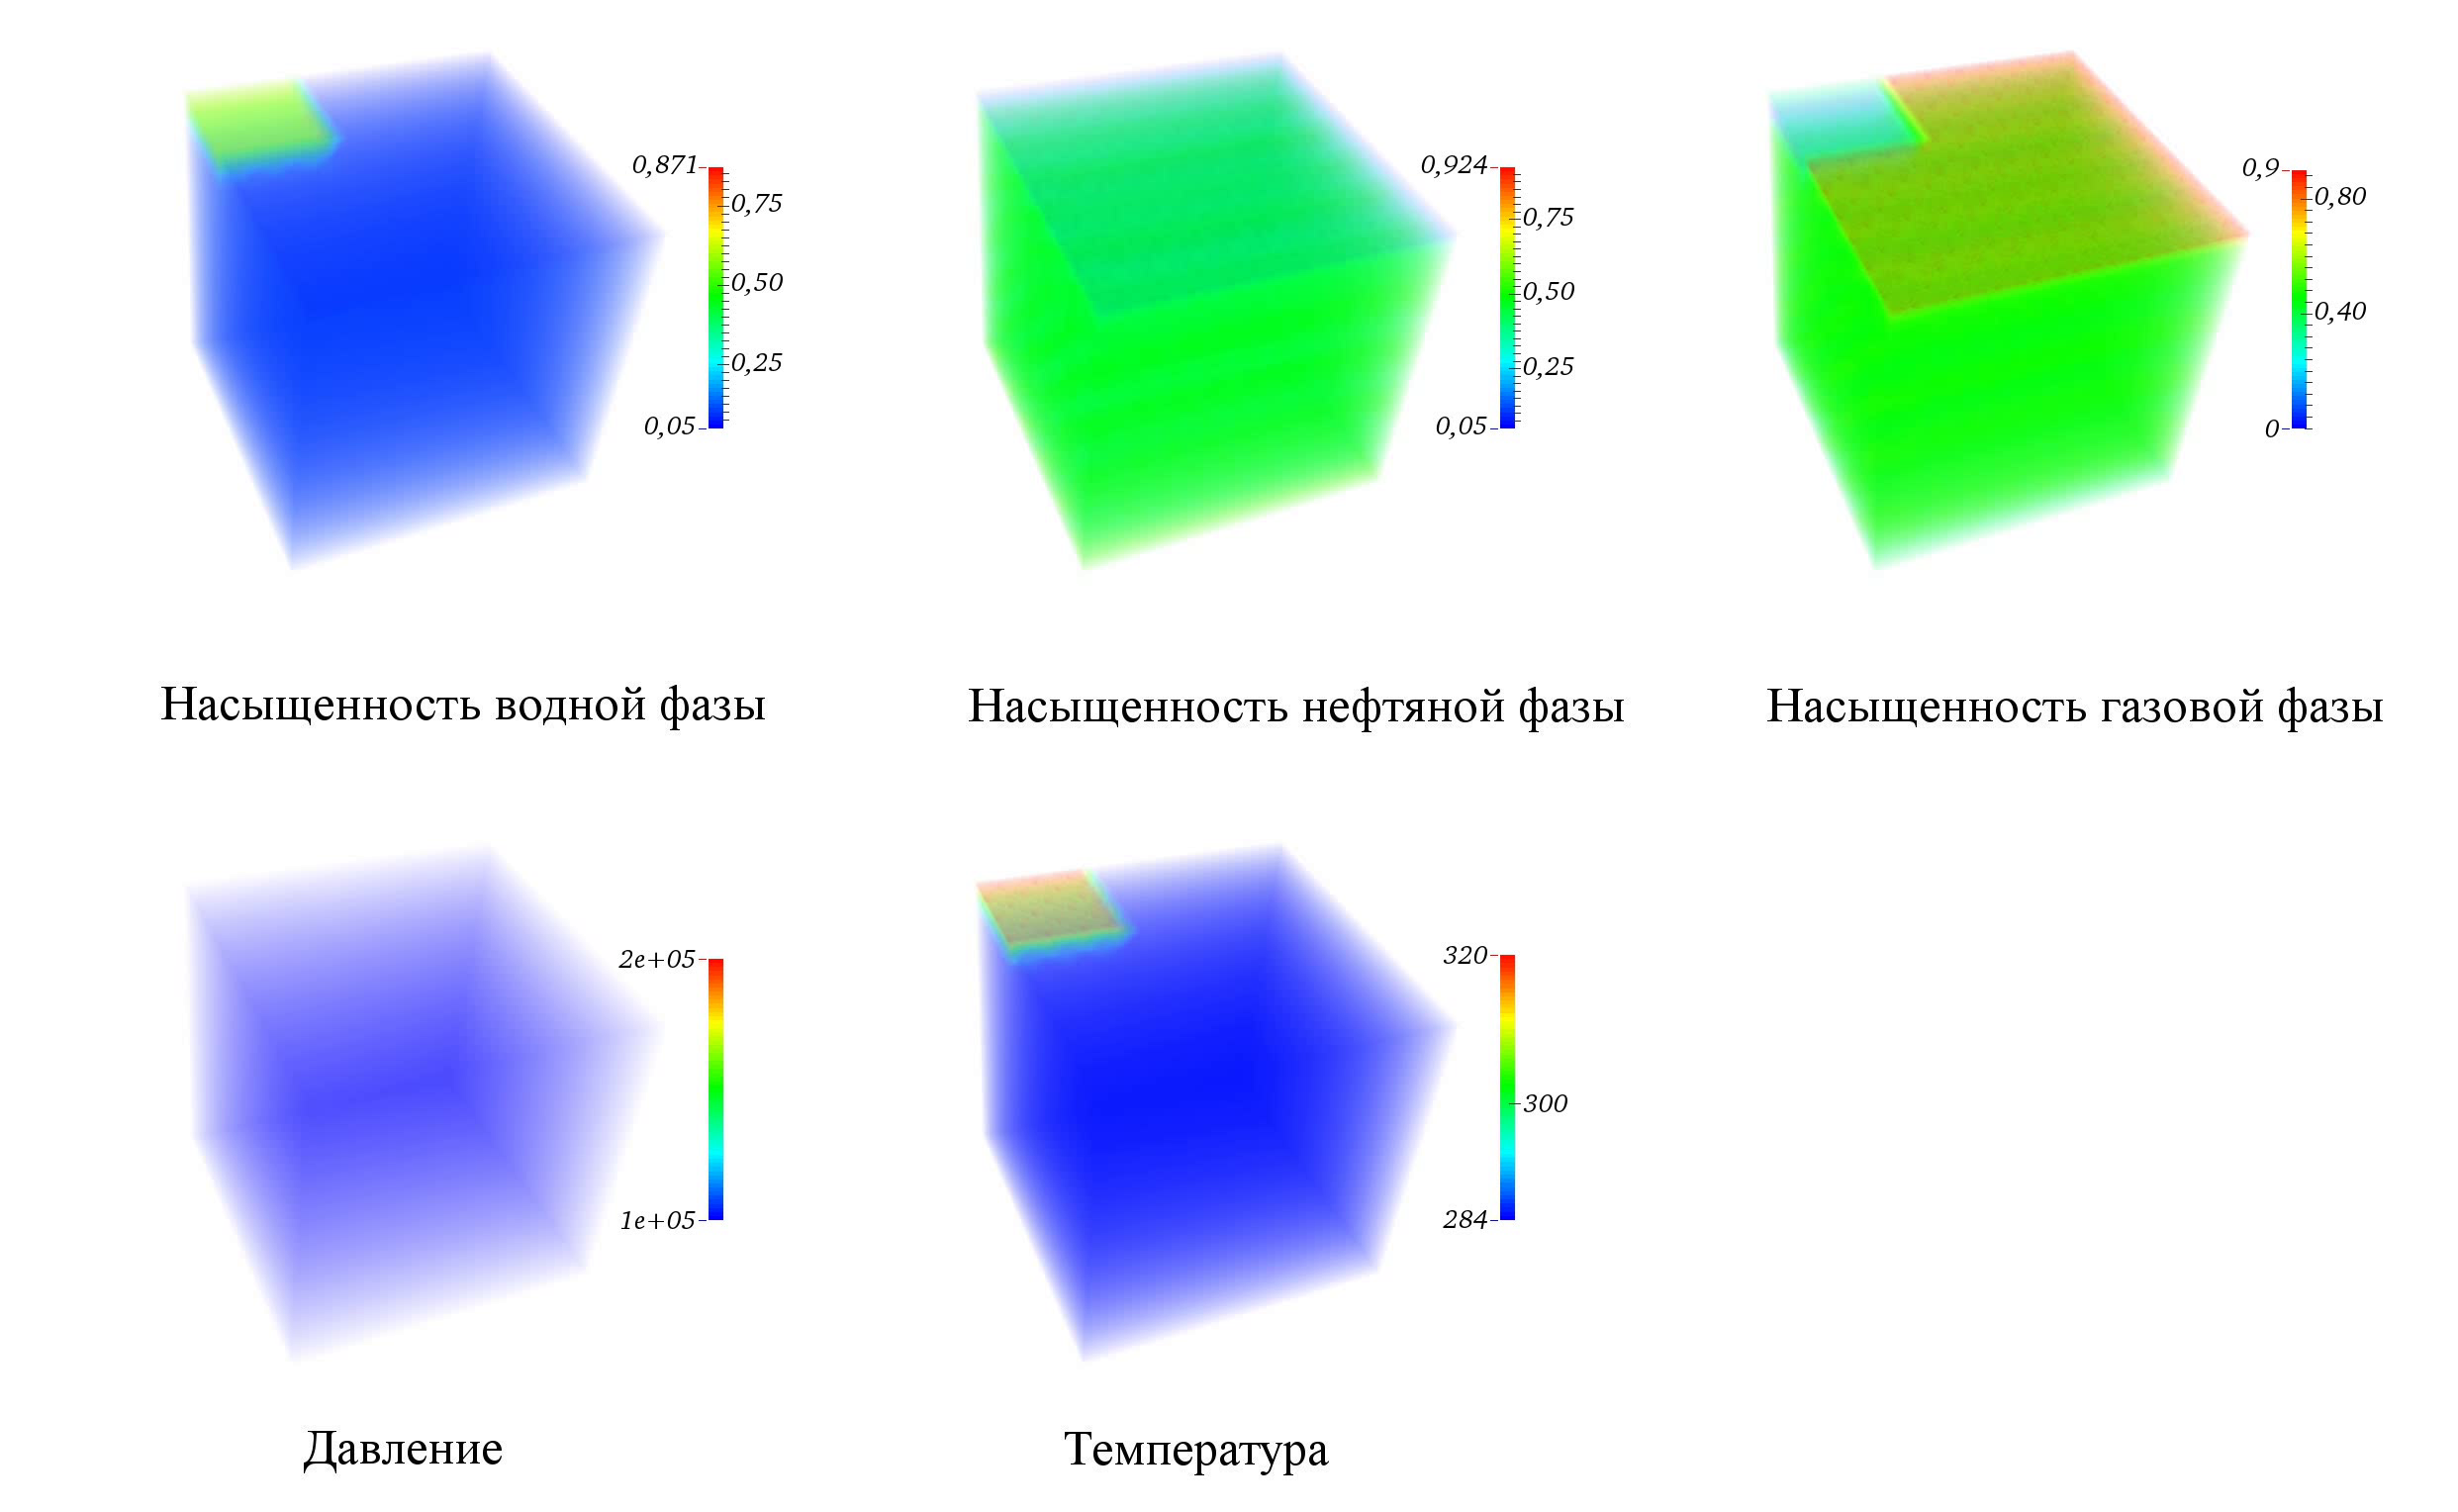
\includegraphics[width=1.0\textwidth]{video/frame.png}}{video/all_full.avi}
\end{figure}
  \end{center}
\end{frame}

\section{Анализ производительности вычислений}

\begin{frame}
\begin{center}
\frametitle{Анализ производительности вычислений}
\framesubtitle{Многопроцессорная система}
\begin{figure}[!h]
\begin{minipage}[h]{0.46\textwidth}
\begin{tikzpicture}
  \begin{axis}[axis lines=left, enlargelimits=true, grid=major, width=1.0\textwidth, height=0.7\textheight, xlabel={\textit{число процессоров}}, ylabel={\textit{ускорение}}]
    \pgfplotstableread{data/mpi_times.txt}{\mytable}
    \pgfplotstablegetelem{0}{Y}\of{\mytable}
    \pgfmathsetmacro{\ay}{\pgfplotsretval}
    \addplot [blue, mark=*] table [x=X, y expr=\ay/\thisrow{Y}] {\mytable};
  \end{axis}
\end{tikzpicture}
%\caption{Зависимость ускорения расчета тестовой задачи от числа процессоров}
\label{mpi_speedup}
\end{minipage}
\hfill
\begin{minipage}[h]{0.46\textwidth}
\begin{tikzpicture}
  \begin{axis}[axis lines=left, enlargelimits=true, grid=major, width=1.0\textwidth, height=0.7\textheight, xlabel={\textit{число процессоров}}, ylabel={\textit{эффективность}}]
    \pgfplotstableread{data/mpi_times.txt}{\mytable}
    \pgfplotstablegetelem{0}{Y}\of{\mytable}
    \pgfmathsetmacro{\ay}{\pgfplotsretval}
    \addplot [blue,mark=*] table [x=X, y expr=\ay/\thisrow{Y}/\thisrow{X}] {\mytable};
  \end{axis}
\end{tikzpicture}
%\caption{Зависимость эффективности расчета тестовой задачи от числа процессоров}
\label{mpi_eff}
\end{minipage}
\end{figure}
\end{center}
\end{frame}

\begin{frame}
\begin{center}
\frametitle{Анализ производительности вычислений}
\framesubtitle{Графический ускоритель}
\begin{figure}[!h]
\begin{center}
\begin{tikzpicture}
  \begin{axis}[axis lines=left, enlargelimits=true, grid=major, width=0.6\textwidth, xlabel={\textit{число узлов сетки}}, ylabel={\textit{ускорение}}]
    \pgfplotstableread[skip first n=1]{data/cpu_vs_gpu.txt}{\mytable}
    \addplot [blue, mark=*] table [x=0, y expr=\thisrow{1}/\thisrow{2}] {\mytable};
  \end{axis}
\end{tikzpicture}
\caption{GPU vs CPU}
\label{cuda_speedup}
\end{center}
\end{figure}
\end{center}
\end{frame}


\section{Заключение}
\begin{frame}
\begin{center}
\frametitle{Заключение}
\framesubtitle{\ }
В процессе работы над дипломом:
\begin{itemize}
  \item предложены 1D, 2D и 3D-модели трехфазных течений в пористых средах;
  \item разработан алгоритм расчета;
  \item алгоритм расчета распараллелен;
  \item написан программный комплекс;
  \item в необходимом объеме освоены технологии MPI, Nvidia CUDA, визуализации данных расчетов;
  \item программный комплекс протестирован на нескольких тестовых задачах 
  фильтрации;
  \item сделаны три доклада на конференциях, одна из которых -- международная;
  \item написаны в соавторстве две статьи.
\end{itemize}
\end{center}
\end{frame}

\begin{frame}
\begin{center}
\frametitle{\ }
\framesubtitle{\ }
\item {\huge Спасибо за внимание!}
\end{center}
\end{frame}

\end{document}
